\documentclass[12pt]{article}
\usepackage{configurado}

\addbibresource{bibliografia.bib}

\title{Un Lenguaje de Programación del Futuro}
\newcommand{\thecurso}{Lenguajes de Programación}
\author{Lucas Lois}
\date{\today}

% 2000 palabras máximo

\begin{document}
\maketitle
%%%%%%%%%%%%%%%%%%%%%%%%%%%%%%%%%%%%%%%%%%%%%%%%%%%%%%%%%%%
\begin{abstract}

En este trabajo se intenta atacar el problema de la creciente complejidad del
software, en cuanto a cómo afecta la capacidad de trabajo del desarrollador,
mediante una serie de principios que puedan guiar la creación de nuevos
lenguajes de programación.
El lenguaje del futuro, para el desarrollo de aplicaciones interactivas, deberá
proveer las abstracciones adecuadas en su sintaxis para facilitar un desarrollo
que debe ser guiado por la ayuda de herramientas de análisis estático de tipos.

\end{abstract}

\section{Introducción}

Las características deseadas de un lenguaje de programación dependen de la
tarea que se espera llevar a cabo con ellos.
Aunque muchos programadores participen de una guerra santa sobre qué lenguaje
de programación es ``el mejor'', esto es un error, ya que se ve al lenguaje
como el fin y no como lo que es, una mera herramienta para el desarrollo de una
solución informática.

Habiendo dicho esto, ahondaremos a continuación en el caso de desarrollo de
aplicaciones interactivas, presentando los problemas presentados en el campo y
derivando algunas características que \emph{el lenguaje del futuro} deberá
tener.

\section{\emph{Syntax Matters}}

En \emph{Deep Work}~\autocite{deepwork}, Newport presenta el caso para un
ambiente de trabajo libre de distracciones para trabajos creativos como la
ingeniería de software, tomando de su propia experiencia profesional.
Newport argumenta que al buscar la creación de sistemas complejos es muy importante
evitar distracciones para poder estar completamente enfocado en la tarea, y
así llegar a lo que el campo \emph{new age} llama ``estado de \emph{flow}''.
El principal punto aquí es que las distracciones frecuentes (e.g.\ en una
oficina de planta abierta) hacen que se interrumpa el complejo proceso de
análisis necesario en un sistema lo suficientemente complejo, no logrando
llegar a un nivel de abstracción que nos permite implementar los cambios
necesarios al código (\autoref{fig:interrupt}).

\begin{figure}[ht]
    \begin{center}
        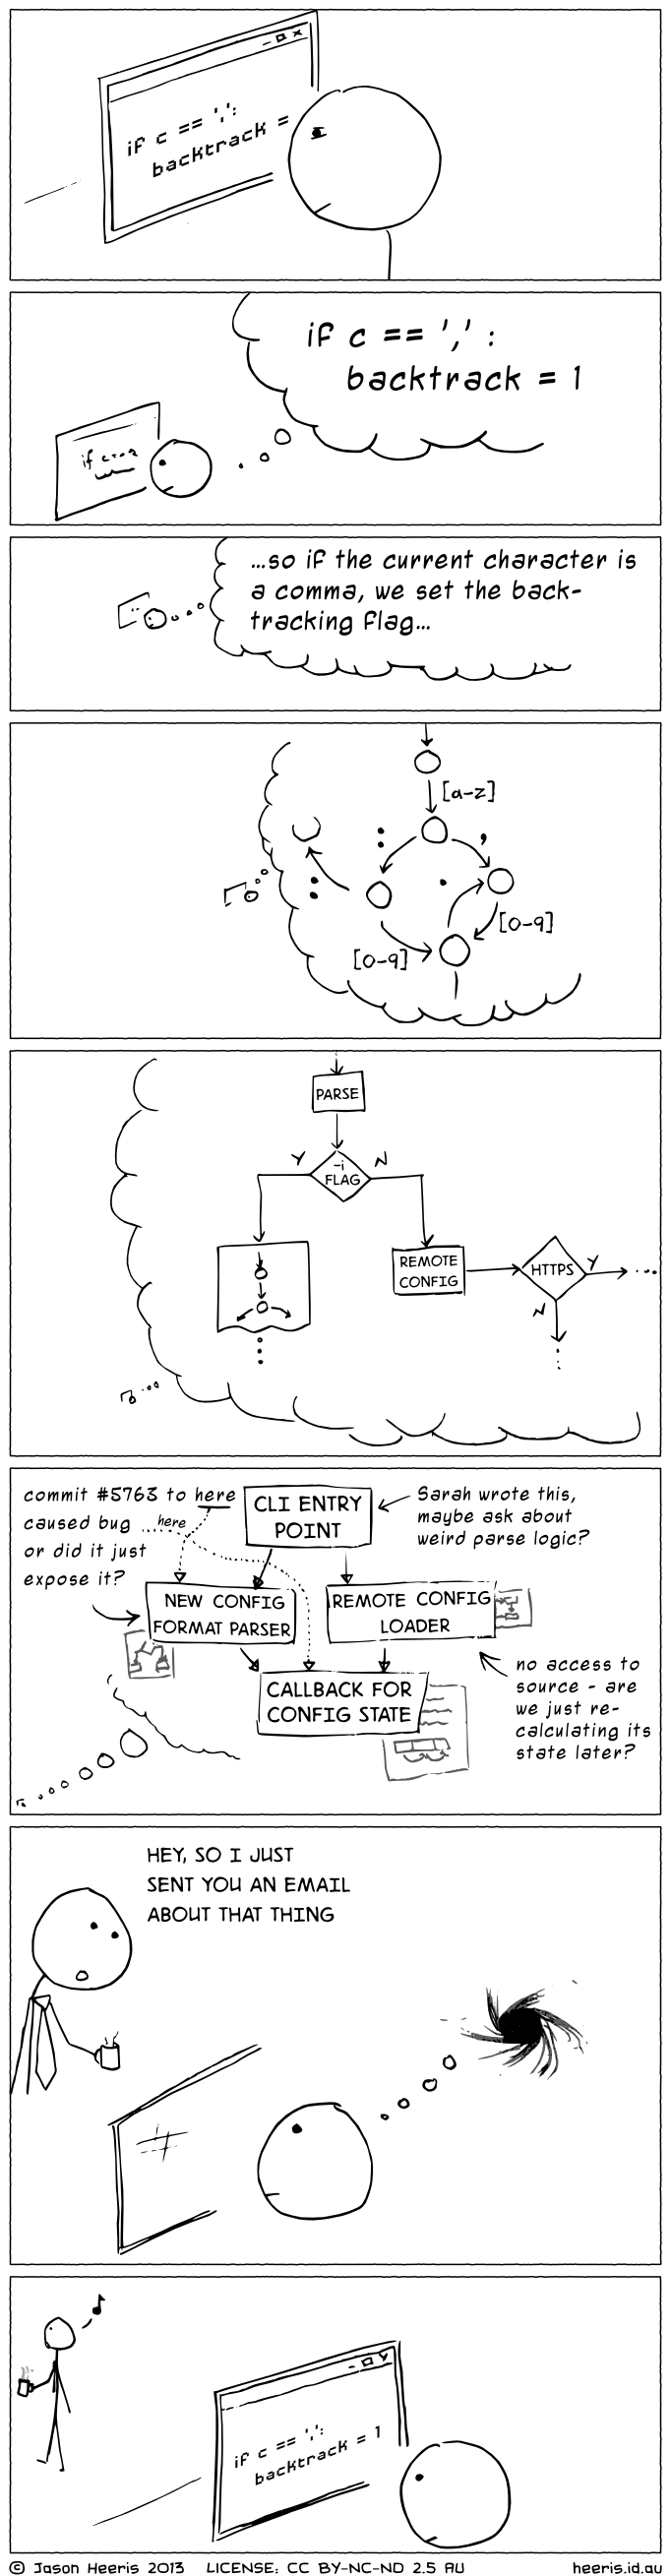
\includegraphics[width=0.4\textwidth]{interrupted}
        \caption{Las interrupciones son un gran problema en el campo del desarrollo}
	\label{fig:interrupt}
    \end{center}
\end{figure}

Entendiendo este problema, ¿es posible que un lenguaje de programación ayude de
alguna forma?
Desde las matemáticas, Terence Tao~\autocite{goodnotation} destaca la
importancia del uso de una buena notación, para ``hacer énfasis en los
parámetros y características más importantes de una expresión, mientras se
minimizan los aspectos cotidianos que no son de interés.''
Los ejemplos en ese campo sobran, de cómo se pueden construir con algunos
símbolos expresiones que abstraen gran complejidad, y un sinnúmero de definiciones
y teoremas por detrás.
Whitehead~\autocite{intromath} va un paso mas allá, afirmando que una notación
concisa, como \(lim_{x\to_0} \sin x = 0\), libera al cerebro del trabajo innecesario
de lidiar con la verdadera
expresión\footnote{\(\forall \epsilon > 0, \exists \delta > 0, (|x| < \delta \Rightarrow |\sin x| < \epsilon)\), aunque esta expresión es también una abstracción, con
los conceptos de \(\sin\), \(0\), valor absoluto, \(\forall\), y demás.}
así dejándolo libre para ``concentrarse en problemas más avanzados, en
efecto incrementando su poder''.

Esta idea es soportada por la literatura. Nielsen~\autocite{augmentingcognition}
presenta el argumento desde la neurociencia, donde estudiando a jugadores de ajedrez
se observa que los mejores jugadores lo son porque lograron \emph{abstraer} el movimiento
de cada pieza y ven patrones de juego. De esta forma logran pensar en menos
elementos disjuntos pero asimismo ver más que un \emph{amateur}.

El concepto de ``fragmento'' de Herbert Simon presentado en ese articulo
sostiene la teoría de que solo podemos trabajar con \(\sim\) 7 de estos ``fragmentos''
en nuestra memoria en cualquier momento dado, y solo es posible lograr el
pensamiento complejo si logramos que cada fragmento tenga en sí más y más
contenido.

La notación (en matemáticas así como en programación) tiene un rol
importantísimo en esto.
Es fácil de entender si vemos lo fácil que es llevar una tarea de inteligencia
artificial utilizando los bloques en una herramienta como Rapid Miner, pero es,
a todos los efectos, imposible de hacer en un \texttt{assembly x86}.
No se trata de un problema de poder, ya que al final del día el programa de
bloques acaba en traducirse a las únicas instrucciones que un procesador
entiende. Se trata sí de la abstracción que nos provee la sintaxis (visual en
el caso), donde cada ``fragmento'' trata explícitamente de tareas relevantes
como \emph{Naive Bayes o PCA}.

React es un claro ejemplo de esto, y su éxito una prueba de su importancia.
Con JSX y el DOM virtual, React~\autocite{flux} (y posteriormente
Elm~\autocite{elmarch}) logró pasar del modelo de interfaces vivas, donde se
tenía que modificar cada pieza que cambia luego de una interacción del usuario,
a uno mucho más simple, donde la interfaz se construye a partir del estado
actual del programa, y se construye desde cero cada vez (o al menos eso parece
a quien lo implementa).
Siguiendo la misma sinfonía, se lleva la misma tarea a cabo por debajo (el
``x86'' de los navegadores nunca cambió, seguimos cambiando elementos de forma
individual), pero se posiciona al programador en un nivel más alto de
abstracción.

La introducción de los \emph{hooks}~\autocite{hooks} llevan este poder
un paso más adelante, ya que con la sintaxis \texttt{useX}, las interfaces
construidas pueden tener valores que cambian a medida que avanza el programa,
como si fueran funciones que devuelven un valor que cambia con el tiempo.
Una vez más, los valores que devuelven son tan inmutables como cualquier otro,
y lo que pasa en realidad es que se llama a la función repetidas veces,
redibujando el componente en cada instancia.

\section{Un compilador que trabaje por nosotros}

Al usar lenguajes como Haskell, con tipos con la suficiente expresividad como
para que el compilador logre guiar la implementación de cada función con tan
solo declarar su tipo~\autocite{typeholes}, el programador logra liberar aún más
su mente de los detalles ``triviales'', que de cierta forma ya están
codificados en los tipos de datos y funciones.
Elm, un lenguaje diseñado para la implementación de \emph{web apps} fuertemente
inspirado en Haskell, logró también un compilador extremadamente útil que colabora
con el programador para llegar a una implementación o completar un refactor.
Feldman~\autocite{elmdatastructure} presenta en su charla cómo el sistema de
tipos es tan capaz que se logra la implementación de una interfaz gráfica
(incluida la interacción del usuario) con gran facilidad partiendo de la
estructura de datos diseñada, siempre y cuando esta modele el dominio
correctamente.

\subsection{Modelo, Funciones y Efectos}

Seemann va un paso mas allá~\autocite{pitofsuccess}, presentando cómo la rigidez
de un lenguaje tipado, que logra separar con claridad los modelos (estructuras
de datos puras) de las funciones (mapas entre tipos de datos pero \emph{sin
efectos secundarios}) y efectos (a su vez restringidos en los distintos
dominios~\autocite{modernfp}), alcanza naturalmente y sin esfuerzo una
arquitectura de ``puertos y adaptadores'', o ``en capas'', correctamente.

Polysemy~\autocite{polysemy} es una librería para el lenguaje Haskell que permite
la declaración de los ``efectos'' de nuestro programa de forma abstracta,
como una estructura de datos, lo que nos permite programar de forma
general en nuestro dominio.
Solo luego se implementan ``intérpretes'', que \emph{traducen estos efectos
acciones en el mundo real} (i.e.\ operaciones de E/S a archivos, consola, red,
etc.).
Esto nace de un concepto llamado ``Mónadas gratuitas''~\autocite{freermonads}.

\begin{lstlisting}[language=Haskell]
data Teletype m a where
  ReadTTY  :: Teletype m String
  WriteTTY :: String -> Teletype m ()
makeSem ''Teletype

echo = do
  i <- readTTY
  writeTTY i
  echo -- Calls echo recursively
\end{lstlisting}

Como se muestra en el ejemplo, el programador define su dominio de acción (como
las capacidades de leer y escribir Strings) y escribe sus programas (como
\texttt{echo}) según esta abstracción.
En \emph{ningún} momento, sin embargo, hace referencia a los detalles sobre si
estas operaciones ocurren con archivos, consola, red, o valores de la memoria.
Una vez más, el modelo mental que se debe mantener está simplificado.
Una vez implementados los detalles de su negocio se pasa a la implementación de
intérpretes, que a su vez son agnósticos a las reglas de lógica del negocio
(e.g. ``luego de cada lectura hacemos una escritura del mismo valor''), que
efectúan esas operaciones en el medio deseado.

Es posible, y deseable, implementar intérpretes de prueba, que leen y escriben
valores predeterminados, fijos, para tener así programas deterministas que pueden
ser probados fácilmente, y no difiere en nada la implementación de un intérprete
así de uno real.
Hemos logrado desacoplar los requisitos del negocio de los problemas de E/S
rutinarios.

Pero hay otra ventaja escondida en esto, y es que el modelo definido (i.e.
Teletype), \emph{limita} al programador en lo que puede hacer.
Una efecto del tipo Teletype no puede eliminar un archivo, abrir una nueva
conexión, o ``lanzar los misiles''~\autocite{missiles}, y esto, chequeado por
el compilador, asegura al programador que no está atacando áreas que no son
responsabilidad del efecto actual.


\section{Mirando hacia el futuro}


El lenguaje del futuro, para el desarrollo de aplicaciones interactivas, deberá
proveer las abstracciones adecuadas en su sintaxis para facilitar un desarrollo
que debe ser guiado por la ayuda de herramientas de análisis estático de tipos.
Tomaremos para ello el lenguaje de Seemann.
Por un lado se tendrá la declaración de interfaces, declaradas como función del
estado, con una sintaxis análoga a JSX (i.e.\ XML), siguiendo una arquitectura
flux~\autocite{flux}.
Los dos elementos de estado, modelo y funciones de actualización, no son mas
que estructuras algebraicas con funciones puras \(A \to M \to M\) que actúan
sobre ellos, con el análisis de tipos asegurando que el modelo es inmutable y
la función de actualización no ejecuta ningún efecto secundario.

Finalmente entra en juego el elemento más importante de este acertijo, y es el
manejo de efectos.
Cada componente de la interfaz debe declarar los efectos que disparará en
respuesta a la interacción, y los tipos lo reflejan, confirmando así en tiempo
de compilación las responsabilidades \emph{totales} de cada componente
en lo que concierne a los efectos ajenos a su visual (esta responsabilidad queda
implícita en el hecho de que lo que se declara es una interfaz).

El efecto primordial es el de despacho, que permite declarar una acción de tipo
\(A\) para operar sobre el modelo \(M\) con las funciones de actualización
descritas anteriormente.  Este efecto es primitivo, y se ofrece al usuario por
parte del lenguaje.
Los demás efectos serán declarados por el usuario o una librería estándar, y
todos se harán de forma abstracta, como en el caso de las mónadas gratuitas,
proveyendo por otro lado los intérpretes necesarios (incluyendo uno de prueba).

Para asegurar el control total en el sistema de tipos de la separación de las
distintas capas se opta por un modelo monádico de las operaciones de E/S, como
en el caso de Haskell, completando así el sistema que asegura una separación
adecuada de las responsabilidades, mientras logra facilitar el modelo mental
del desarrollador y funcionando como asistente para la implementación.

A continuación se presenta una forma primitiva de este lenguaje, para ilustrar
los conceptos.

\begin{lstlisting}[language=Haskell]
-- Los efectos deben declararse como tales.
effect Logging =
  WriteToTheLog :: String -> Logging ()

-- Se declara el tipo de la estructura con su valor inicial
model Counter: Int = 0

action IncrementCounter :: ()

response Counter to IncrementCounter where
  IncrementCounter count = count + 1

-- La declaracion de una GUI requiere modelo y efectos relevantes
gui Button<Counter, Logging> = (counter) => {
  return (
    <button onPress={() => Dispatch(IncrementCounter)}>
      {counter}
    </button>
  )
}

-- se declaran aqui las acciones de este efecto en el mundo
implementation Loggin where
  WriteToTheLog = ...
\end{lstlisting}


%%%%%%%%%%%%%%%%%%%%%%%%%%%%%%%%%%%%%%%%%%%%%%%%%%%%%%%%%%%
\printbibliography{}
\end{document}
